\documentclass{article}
\usepackage{amsmath, amssymb, amsthm, algorithm, algpseudocode, hyperref}
\usepackage{geometry}
\usepackage{etoolbox}
\usepackage{graphicx}
\usepackage{float}

\title{\LARGE CS-5211: Advanced Algorithms \\ \Large Project: Efficient Matrix Multiplication on GPUs}
\author{Rushil Gupta}
\date{\today}

\begin{document}

\maketitle

\tableofcontents

\vspace{0.5in}
\section{Introduction}
In this paper, we explore the architecture of modern GPUs, specifically the Tesla architecture by NVIDIA, and build efficient matrix multiplication algorithms from the ground up. Matrix multiplication is a fundamental operation in many scientific computing and machine learning applications, and optimizing it for GPUs can lead to significant performance improvements. We begin by discussing the GPU model and its key features, followed by a comparison with the classical PRAM model. We then present a variety of matrix multiplication algorithms, starting from a naive approach and progressing to more sophisticated techniques that leverage the GPU architecture effectively.


\vspace{0.5in}
\section{The GPU Model}
In this paper, we will restrict our discussion to the Tesla architecture framework by NVIDIA. A Tesla GPU consists of an array of streaming multi-processors (SMs), each with eight processor cores and a shared memory. These cores are connected to global memory through an interconnection network. The global memory is arranged in independent memory partitions. The interconnection network routes the read/write memory requests from the processor cores to the respective memory partitions, and the results back to the cores. Each memory partition has its own queue for memory requests and arbitrates among the incoming read/write requests. Figure \ref{fig:gpu_architecture} shows the architecture of a Tesla GPU. We now discuss some key ideas in the GPU model.

\begin{figure}[h]
    \centering
    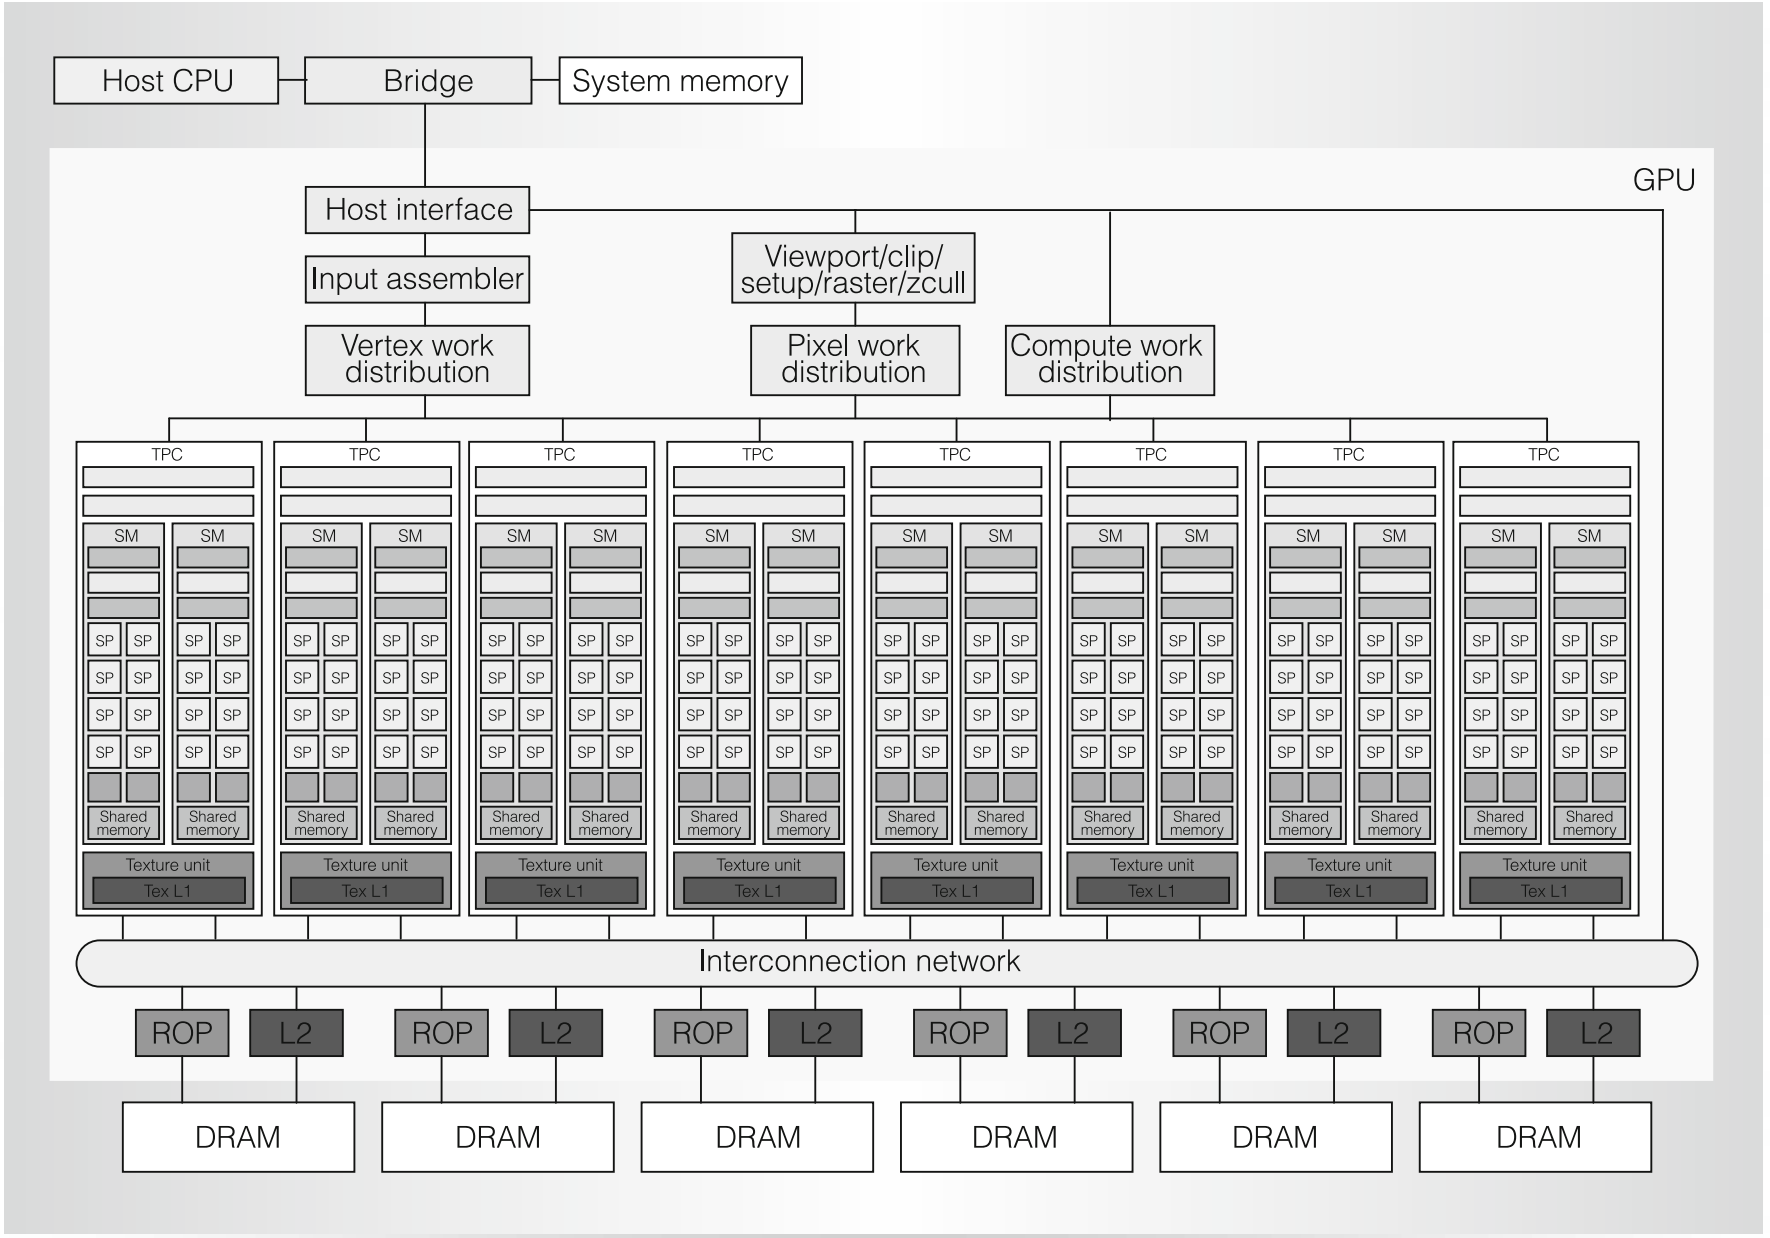
\includegraphics[width=0.8\textwidth]{gpu_architecture.png}
    \caption{Tesla GPU Architecture \cite{ELindholm2008}}
    \label{fig:gpu_architecture}
\end{figure}

\textbf{Concurrent Memory Access.} As mentioned earlier, the entire global memory is accessible to all processor cores through the interconnection network, which routes memory requests to the appropriate memory partitions. Each memory partition has its own queue for incoming memory requests, and is responsible for arbitrating among these requests. The concurrent writes are executed arbitrarily: one of the writes is chosen and the others are ignored. Concurrent reads are supported as well, and it is almost obvious that concurrent writes and reads are not recommended since they can cause race conditions.

\textbf{SIMT Thread Allocation.} GPUs adopt the SIMT (Single Instruction Multiple Thread) model of parallelism. The large idea of the model is for the programmer to specify thread level code for independent threads as well as data-parallel code for coordinated threads. Then, a large number of threads are executed in parallel, with each thread executing the same instruction but on different data. In the Tesla architecture, all threads are divided into ``blocks'' of upto 768 threads each. Each block is assigned to a single SM. An SM executes a thread block by breaking it into groups of 32 threads called warps and executing them in parallel using its eight cores.

There is an important point that needs to be addressed here: branch conditions. Although each thread in a warp executes the same instruction, it is possible that some threads may take different branches in the code. In such cases, the warp serially executes each branch path taken by any thread in the warp, disabling threads that are not on that path. This can lead to significant performance degradation if many threads in a warp take different branches. However, discussing this in detail is beyond the scope of this paper.

\textbf{Thread Synchronization.} The threads by default are not synchronized. However, threads within a block can be synchronized using inbuilt synchronization primitives. However, there is no way to synchronize threads across different blocks. To counter this, programmers can divide their computation into multiple kernel invocations (kernels are the functions executed on the GPU). So once a kernel finishes executing, all threads are synchronized before the next kernel is invoked.

\textbf{Kernels.} A kernel is a function that is executed on the GPU. The programmer specifies the number of blocks and the number of threads per block when invoking a kernel. Each thread has its own unique thread ID, which can be used to access different data elements. The threads within a block can communicate with each other using shared memory. When the program is run, a CPU program first copies the data from the host memory to the global memory of the GPU. Then, it invokes the kernel on the GPU, specifying the number of blocks and threads per block. Once the kernel finishes executing, the CPU program copies the results back from the global memory of the GPU to the host memory.

\vspace{0.2in}
\subsection{Comparison with the PRAM model}
The PRAM model is a classical theoretical model used widely in algorithm design. GPUs and PRAM are similar in the sense that GPUs support a large number of parallel threads, much like the PRAM model. In fact, most modern GPUs require a large number of threads to fully utilize the hardware and hide latency. From our discussion of the GPU model, we can see that the PRAM model related most closely to GPUs is the CRCW-PRAM model (concurrent read, concurrent write).

However, there are some important distinctions that need to be made. First, the PRAM model assumes that all memory accesses take unit time, which is not true in practice. In GPUs, memory accesses can take varying amounts of time depending on factors such as access patterns, memory hierarchy, and contention. Accessing global memory is the most expensive operation, which is orders of magnitude slower than accessing shared memory. Similarly, accessing shared memory is slower than accessing registers. Second, the PRAM model assumes that there is no overhead for thread management and synchronization, which is also not true in practice. In GPUs, there is overhead associated with launching threads, managing warps, and synchronizing threads within a block.


\vspace{0.5in}
\section{GEMM GPU Implementation}
\subsection{Naive Approach}
We first discuss the efficient implementation of matrix multiplication on GPUs, which is a key operation in neural network training. The naive approach to matrix multiplication involves each thread computing a single element of the output matrix by performing a dot product of the corresponding row and column. A pseudocode for the naive approach is given below:

\begin{algorithm}[H]
\caption{Naive Matrix Multiplication on a GPU}
\begin{algorithmic}
    \State \textbf{CPU Code:}
    \State \quad Copy matrices \(\texttt{A}\) and \(\texttt{B}\) to GPU global memory.
    \State \quad Specify the thread blocks. Each thread is assigned a unique \((\texttt{row}, \texttt{col})\) index.
    \State \quad Launch kernel to compute \(\texttt{C} = \texttt{A} \times \texttt{B}\).
    \State \quad Copy result matrix \(\texttt{C}\) back to CPU memory.

    \vspace{\baselineskip}

    \State \textbf{GPU Kernel:}
    \State \quad Get unique thread index \((r, c)\).
    \State \quad Initialize \(\texttt{sum} \gets 0\).
    \State \quad \textbf{for } \(k = 0 \ \textbf{to}\ \texttt{cols(A)} - 1\) \textbf{ do}
    \State \quad \quad \(\texttt{sum} \gets \texttt{sum} + \texttt{A}[r][k] \cdot \texttt{B}[k][c]\)
    \State \quad \textbf{end for}
    \State \quad \(\texttt{C}[r][c] \gets \texttt{sum}\)
\end{algorithmic}
\end{algorithm}

However, this naive approach does not take advantage of the GPU architecture effectively: it accesses the global memory multiple times for each element of the output matrix, leading to high latency and low throughput. To analyse this, see that we spawn $N^2$ threads, and each thread performs $N$ global memory accesses to read elements of matrices A and B. This results in a total of $O(N^3)$ global memory accesses, which is inefficient. An important remark here is that in the PRAM model, this naive approach would be optimal since all memory accesses take unit time. However, in the GPU model, we need to optimize memory accesses to achieve better performance.

\vspace{0.2in}
\subsection{Tiled Matrix Multiplication}
We now discuss the ``tiling'' approach, which improves memory access patterns and utilizes shared memory to reduce global memory accesses. The key observation is that the same elements of the input matrices are fetched multiple times when computing different elements of the output matrix. By loading these elements into shared memory, we can reduce the number of global memory accesses significantly. We first define the notion of a ``tile''. A tile is a sub-matrix of the input matrices that fits into shared memory of an SM. Let $k$ denote the tile size. Figure \ref{fig:matrix_tiling} illustrates the tiles of the output matrix, and the corresponding tiles of the input matrices.

\begin{figure}[H]
    \centering
    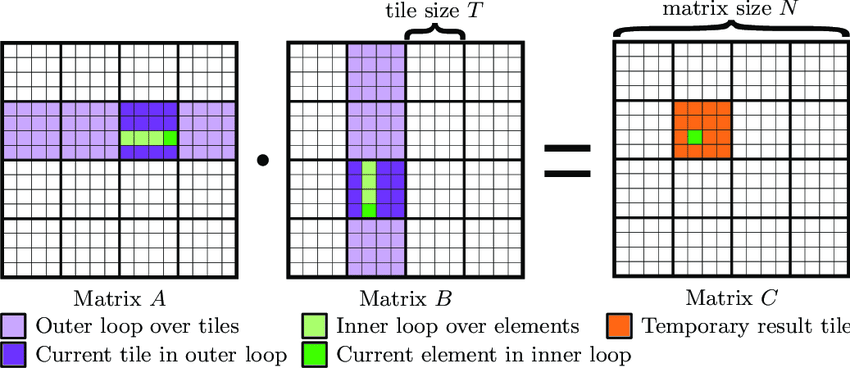
\includegraphics[width=0.8\textwidth]{matrix_tiling.png}
    \caption{Matrix Tiling for Efficient Multiplication \cite{AMatthes2017}}
    \label{fig:matrix_tiling}
\end{figure}

We now describe the algorithm in detail. Consider the $16 \times 16$ output matrix shown in Figure \ref{fig:matrix_tiling}, and let the tile size be $4$. The output matrix is divided into $4 \times 4$ tiles, and a thread block is assigned to compute each tile. Within each thread block, to compute the entires of the tile it is assigned, we allocate 16 threads, where each thread is responsible for computing one element of the $4 \times 4$ output tile. 

\textbf{Thread Computation:} The computation is divided into multiple ``load'' and ``compute'' phases. In the load phase, we load the first $4 \times 4$ tile from matrices $A$ and $B$ into shared memory. This is done cooperatively by all threads in the block - each thread loads one element from each tile of $A$ and $B$ into shared memory, and then synchronizes. After synchronization, each thread only made 1 memory request to global memory, yet has access to all 16 elements of the tiles in shared memory of the SM. Next, in the ``compute phase'', each thread computes a partial sum for its corresponding entry in the output tile using the elements in shared memory (refer to figure \ref{fig:matrix_tiling} for more insight: the green row of the tile in $A$ and the green column of the tile in $B$ are used to partially compute the green element in the output tile of $C$). After the compute phase, we enter the next load phase, where we repeat the same process for the next tiles in $A$ and $B$. Refer to algorithm \ref{alg:tiled_matrix_multiplication} for the complete pseudocode.

\textbf{Analysis:} We first compute the number of memory accesses to compute a single tile in $C$. To compute a single tile, we need to load $\frac{2N}{k}$ tiles from $A$ and $B$ combined. Each tile has $k^2$ elements, and each element is loaded once from global memory. Thus, the total number of global memory accesses to compute a single tile in $C$ is:
\[ \text{Global Memory Accesses per Tile} = \frac{2N}{k} \cdot k^2 = 2Nk \]
Since there are $\frac{N^2}{k^2}$ tiles in $C$, the total number of global memory accesses to compute the entire output matrix $C$ is:
\[ \text{Total Global Memory Accesses} = \frac{N^2}{k^2} \cdot 2Nk = \ \frac{2N^3}{k} \]

So if $W$ is comparable to $N$, we get a huge speedup from the naive approach. A note here is that due to what is called ``memory coalescing'' in GPUs, the constant is not $2$, but is $\frac{1}{16}$.

\begin{algorithm}[H]
\caption{Tiled Matrix Multiplication on a GPU}
\label{alg:tiled_matrix_multiplication}
\begin{algorithmic}
    \State \textbf{CPU Code:}
    \State \quad Copy matrices \(\texttt{A}\) and \(\texttt{B}\) to GPU global memory.
    \State \quad Specify the thread blocks. Each block is assigned a unique \((\texttt{tileRow}, \texttt{tileCol})\) index.
    \State \quad Specify the threads in the block. Each thread is assigned a unique \((\texttt{row}, \texttt{col})\) index.
    \State \quad Launch kernel to compute \(\texttt{C} = \texttt{A} \times \texttt{B}\).
    \State \quad Copy result matrix \(\texttt{C}\) back to CPU memory.

    \vspace{\baselineskip}
    \State \textbf{GPU Kernel:}
    \State \quad \(\texttt{tileRow}, \texttt{tileCol} \gets\) the index of the tile this block is assigned to.
    \State \quad \(\texttt{row}, \texttt{col} \gets\) the index of the tile this thread is assigned to.
    \State \quad Initialize \(\texttt{sum} \gets 0\).
    \State \quad Declare shared memory arrays \(A_{\texttt{sub}}[k][k]\) and \(B_{\texttt{sub}}[k][k]\).
    \State \quad Set \(\texttt{numTiles} \gets \texttt{cols(A)} / k\).

    \vspace{0.5\baselineskip}
    \State \quad \textbf{for } \(t = 0 \ \textbf{to}\ \texttt{numTiles} - 1\) \textbf{ do}
    \State \quad \quad \textbf{Load Phase:}
    \State \quad \quad \quad $A_{\texttt{sub}}[\texttt{row}][\texttt{col}] \gets A[\texttt{tileRow} \cdot k + \texttt{row}][t \cdot k + \texttt{col}]$
    \State \quad \quad \quad $B_{\texttt{sub}}[\texttt{row}][\texttt{col}] \gets B[t \cdot k + \texttt{row}][\texttt{tileCol} \cdot k + \texttt{col}]$
    \State \quad \quad \quad Synchronize threads in the block.

    \vspace{0.5\baselineskip}
    \State \quad \quad \textbf{Compute Phase:}
    \State \quad \quad \quad \textbf{for } \(i = 0 \ \textbf{to}\ k - 1\) \textbf{ do}
    \State \quad \quad \quad \quad \(\texttt{sum} \gets \texttt{sum} + A_{\texttt{sub}}[\texttt{row}][i] \cdot B_{\texttt{sub}}[i][\texttt{col}]\)
    \State \quad \quad \quad \textbf{end for}
    \State \quad \quad \quad Synchronize threads in the block.
    \State \quad \textbf{end for}
    \vspace{0.5\baselineskip}
    \State \quad \(\texttt{C}[\texttt{row}][\texttt{col}] \gets \texttt{sum}\)

\end{algorithmic}
\end{algorithm}

\vspace{0.2in}
\subsection{Thread Coarsening}
In algorithm \ref{alg:tiled_matrix_multiplication}, each thread computes a single element of the output tile by accessing the shared memory of the SM. However, accessing the shared memory is a much more expensive operation when compared to using registers. Thus, we can further optimize the algorithm by allowing each thread to compute multiple elements of the output tile in a way where we can reuse values stored in registers. This technique of merging the work of multiple threads into a single thread is called ``thread coarsening''.

The change we make is that instead of each thread computing a single element of the output tile, each thread computes $\texttt{WPT}$, which stands for `work per thread', elements of the output tile. The key gain comes in the compute phase. Instead of loading the entires of the appropriate rows of $A_{\texttt{sub}}$ and columns of $B_{\texttt{sub}}$ from shared memory multiple times, in the new inner-most loop, we load one entry of $A_{\texttt{sub}}$ into a register, and reuse it to compute multiple elements of the output tile. The pseudocode for the modified kernel is given in algorithm \ref{alg:thread_coarsened_tiled_matrix_multiplication}.

\begin{algorithm}[H]
\caption{Tiled Matrix Multiplication with Thread Coarsening on a GPU}
\label{alg:thread_coarsened_tiled_matrix_multiplication}
\begin{algorithmic}
    \State \textbf{GPU Kernel:}
    \State \quad \(\texttt{tileRow}, \texttt{tileCol} \gets\) the index of the tile this block is assigned to.
    \State \quad \(\texttt{row}, \texttt{col} \gets\) the index of the tile this thread is assigned to.
    \State \quad Declare shared memory arrays \(A_{\texttt{sub}}[k][k]\) and \(B_{\texttt{sub}}[k][k]\).
    \State \quad Initialize \(\texttt{sum}[0..\texttt{WPT}-1] \gets 0\).
    \State \quad Set \(\texttt{numTiles} \gets \texttt{cols(A)} / k\). 

    \vspace{0.5\baselineskip}
    \State \quad \textbf{for } \(t = 0 \ \textbf{to}\ \texttt{numTiles} - 1\) \textbf{ do}
    \State \quad \quad \textbf{Load Phase:}
    \State \quad \quad \quad $A_{\texttt{sub}}[\texttt{row}][\texttt{col}] \gets A[\texttt{tileRow} \cdot k + \texttt{row}][t \cdot k + \text{col}]$
    \State \quad \quad \quad $B_{\texttt{sub}}[\texttt{row}][\texttt{col}] \gets B[t \cdot k + \texttt{row}][\texttt{tileCol} \cdot k + \texttt{col}]$
    \State \quad \quad \quad Synchronize threads in the block.
    \State \quad \quad \textbf{Compute Phase:}
    \State \quad \quad \quad \textbf{for } \(i = 0 \ \textbf{to}\ k - 1\) \textbf{ do}
    \State \quad \quad \quad \quad $a_{\texttt{reg}} \gets A_{\texttt{sub}}[\texttt{row}][i]$ \Comment{Load into register once}
    \State \quad \quad \quad \quad \textbf{for } \(j = 0 \ \textbf{to}\ \texttt{WPT} - 1\) \textbf{ do}
    \State \quad \quad \quad \quad \quad \(\texttt{sum}[j] \gets \texttt{sum}[j] + a_{\texttt{reg}} \cdot B_{\texttt{sub}}[i][\texttt {col} + j \cdot \texttt{blockDim.y}]\) \Comment{Reuse register value}
    \State \quad \quad \quad \quad \textbf{end for}
    \State \quad \quad \quad \textbf{end for}
    \State \quad \quad \quad Synchronize threads in the block.
    \State \quad \textbf{end for}

    \vspace{0.5\baselineskip}
    \State \quad \textbf{for } \(j = 0 \ \textbf{to}\ \texttt{WPT} - 1\) \textbf{ do}
    \State \quad \quad \(\texttt{C}[\texttt{row}][\texttt{col} + j \cdot \texttt{blockDim.y}] \gets \texttt{sum}[j]\)
    \State \quad \textbf{end for}
\end{algorithmic}
\end{algorithm}

\textbf{Analysis:} The total number of global memory accesses remains the same as in the previous tiling approach, which is $\frac{2N^3}{k}$. However, we have reduced the number of shared memory accesses significantly. In the previous approach, each thread accessed shared memory $k$ times in the compute phase. Now, each thread accesses shared memory only $\frac{k}{\texttt{WPT}}$ times in the compute phase, since it reuses values stored in registers. This leads to a significant performance improvement, especially for larger tile sizes and higher work per thread values.

\vspace{0.2in}
\subsection{Memory Coalescing}
The last optimisation we present is the use of larger data types to improve memory bandwidth utilization. Instead of loading each element of the tiles from global memory individually, we can load multiple elements at once using larger data types such $\texttt{float8}$. The key idea is that global memory accesses are more efficient when they are coalesced, i.e., when multiple contiguous memory locations are accessed in a single transaction. By using larger data types, we can load multiple elements of the tiles in a single global memory access, thereby reducing the total number of global memory accesses. This is called ``memory coalescing''.

We do not present the pseudocode for this optimisation, as it is a straightforward modification to the load phase of the previous algorithms. Instead of loading a single element from global memory, we load multiple elements using larger data types. The analysis remains the same as before, but with a reduced constant factor in the total number of global memory accesses.

\vspace{0.5in}
\section{Conclusion}
In this paper, we explored the architecture of modern GPUs and developed efficient matrix multiplication algorithms that leverage the GPU architecture effectively. We began with a naive approach and progressively introduced optimizations such as tiling, thread coarsening, and memory coalescing. Each of these optimizations significantly improved the performance of matrix multiplication on GPUs by reducing global memory accesses and improving memory bandwidth utilization. There are many more optimizations and techniques that can be applied to further improve the performance of matrix multiplication on GPUs. However, discussing these in detail is beyond the scope of this paper. Overall, the techniques presented in this paper provide a solid foundation for understanding how to optimize matrix multiplication on GPUs, and these ideas can be extended to other parallel algorithms on GPUs as well.

Another key point to be noted is that the architecture discussed in this paper is NVIDIA's Tesla architecture. Over the years, GPU architectures have evolved significantly, with newer architectures introducing additional features and optimizations. The reason we did not discuss these newer architectures is: (i) to keep the scope of the paper manageable, and (ii) because the Tesla architecture provides a solid foundation for understanding GPU programming concepts.

\newpage
\addcontentsline{toc}{section}{References}
\bibliographystyle{plain}
\bibliography{references}
\nocite{*}

\end{document}